\documentclass[12pt,a4paper]{article}
\usepackage[fleqn]{amsmath}
\usepackage[TS1,T2A]{fontenc}
\usepackage{cmap}
\usepackage[left=3cm,right=2.5cm,top=2cm,bottom=2cm,bindingoffset=0cm, headsep=1cm, footskip=1cm]{geometry}
\usepackage[utf8]{inputenc}
\usepackage[english, russian]{babel}
\usepackage{amsfonts}
\usepackage{amssymb}
\usepackage{pdfpages}
\usepackage{slashbox}
\usepackage{graphicx}
\usepackage{mathrsfs}
\usepackage{color}
\usepackage{wrapfig}
\usepackage{multirow}
\usepackage{verbatim}
\usepackage{alltt}
\usepackage{tikz}
\definecolor{blue_repl}{RGB}{0,0,200}
\usepackage[unicode=true, bookmarks=true,bookmarksnumbered=true,bookmarksopen=false, breaklinks=false,pdfborder={0 0 0},backref=section,colorlinks=true,urlcolor=blue_repl,menucolor=blue_repl,linkcolor=blue_repl,citecolor=blue_repl]{hyperref}
\renewcommand*{\backref}[1]{}
\renewcommand{\contentsname}{Title}
\newcommand{\pluseq}{\mathrel{{+}{=}}}

\DeclareMathOperator{\divergence}{div}
\renewcommand{\div}{\divergence}
\DeclareMathOperator{\mes}{mes}
\def\Div{\mathop{\rm div}\nolimits}
%\def\Bold#1{\textbf{\emph{#1}}

% Включать подсекции в оглавление
\setcounter{tocdepth}{2}

\hypersetup{
pdftitle={Diplom},
}

\usepackage[all]{hypcap}
\begin{document}

\includepdf[pages=1]{title.pdf}

\tableofcontents
\newpage
\section{Постановка задачи}
\subsection {Введение}
Рассматривается математическая модель фильтрации вязкой сжимаемой смеси в пористой среде с учетом явления пространственной диффузии. Целью данной работы является численная реализация этой математической модели на параллельных ЭВМ.
\subsection{Задачи}
\begin {itemize}
\item Реализовать модель пространственной диффузии, описываемой законом Фика.
\item Реализовать модель диффузии, применяемой в модели метана угольных пластов.
\end {itemize}

\section{Классическая модель диффузии}

\subsection{Физическая модель}

	Диффузия представляет собой процесс на молекулярном уровне и определяется случайным характером движения отдельных молекул. Она необходима для моделирования задач с низкой проницаемостью среды.

\subsection{Математическая модель}

Задачу фильтрации решают с использованием следующих
 уравнений изотермической композиционной модели (см. например ~\cite{Aziz}, ~\cite{Chen}): 

\label{system_equations}

\begin{eqnarray}
  \label{filtration_1}
  \dfrac{\partial}{\partial t} \left(\phi N_c\right) &=
  & \Div\sum\limits_{P = O, W, G} x_{c,P} \xi_P \Bigl({\bf k} \dfrac{k_{rP}}{\mu_P}(\nabla p_P - \gamma_P \nabla D)\Bigr)+ q_c, \quad c=1,\dots,n_c \qquad \\
  \label{filtration_2}
  p_o - p_g &= &P_{cog}, \\
  \label{filtration_3}
  p_o - p_w &= &P_{cow}, \\
  \label{filtration_4}
  S_w + S_o + S_g &= &1 
\end{eqnarray}

На внешней границе резервуара ставятся условия 
непротекания (однородные условия Неймана).
Начальные условия вычисляются либо по заданным значениям $S_p$, $N_c$, $p$, $x_{c,P}$
(например, от предыдущего расчета),
либо из условий гидростатического равновесия.
Здесь:
\begin{itemize}
\item $n_c$ -- количество компонент, присутствующих в данной задаче. Модели, в которых присутствуют только 3 основные компоненты (вода, нефть, газ), получили название "моделей черной нефти". Модели с большим количеством компонент называются "композиционными моделями". \label{model_types}
\item $N_c=N_c(t,x,y,z)$ (\textbf{неизвестна}) -- $c=1,\ldots, n_c$
молярная плотность компонента.
$$
  N_c=\sum\limits_{P = O, W, G}x_{c,P}\xi_PS_p,
$$
Обозначим ${\bf N} = (N_1, N_2, ... N_{n_c})$
\item $S_p=S_p(t,x,y,z)$ (\textbf{неизвестна}) -- насыщенность $p$-ой фазы, $p=o,g,w$,
\item $p_w=p_w(t,x,y,z)$, $p_o=p_o(t,x,y,z)$, $p_g=p_g(t,x,y,z)$ (неизвестны)
 -- давление в фазах вода, нефть, газ,
\item $\phi=\phi(p_p, x,y,z)$ -- пористость,
\item $x_{c,P} = x_{c,P}(p, \bf N)$ -- молярная доля компонента  $c$ в фазе $P$,
\item $\xi_P = \xi_P(p, \bf N)$ -- молярная плотность фазы,
\item ${\bf k}={\bf k}(p_w,p_o,p_g,x,y,z)$ -- тензор абсолютной проницаемости,
\item $k_{rp}=k_{rp}(S_w,S_g)$ -- относительная фазовая проницаемость,
\item $\mu_p = \mu_p(p_p)$ -- вязкость фазы,
\item $\gamma_p = \rho_p g$ -- вертикальный градиент давления,
\item $D = D (x, y, z)$ -- вектор глубины (сверху вниз),
\item $\rho_p = \rho_p(p_p)$ -- массовая плотность фазы,
\item $q_c = q_c (p, \bf N, t, x, y, z)$ -- источник компонента $c$ (скважина),

\end{itemize}


Диффузия описывается законом Фика: (см. ~\cite{Fick})
\begin{eqnarray}
\label{Fick}
J = cD\nabla j
\end{eqnarray}

\begin{itemize}
\item $J$ -- диффузионный поток в единицу площади
\item $D$ -- коэффициент диффузии
\item $j$ -- потенциал
\end{itemize}
Для многофазных сред движущим потенциалом в законе Фика принято считать разницу концентраций компоненты внутри одной фазы:
$$
J_c = \sum\limits_{P = O, W, G}{c_PD_{c,P}\nabla x_{c,P}}
$$
\begin{itemize}
\item $c_P$ -- молярная концентрация фазы, $c_P = \phi S_p\xi_p$
\item $D_{c,P}$ -- коэффициент диффузионного потока компоненты $c$ в фазе $P$
\item $J_c$ -- диффузионный поток компоненты c в единицу площади
\end{itemize}
Таким образом, уравнение сохранения массы с учетом диффузионных перетоков перепишется в виде:
\begin{eqnarray}
\dfrac{\partial}{\partial t} \left(\phi N_c\right) &=
  & \Div\sum\limits_{P = O, W, G} x_{c,P} \xi_P \Bigl({\bf k} \dfrac{k_{rP}}{\mu_P}(\nabla p_P - \gamma_P \nabla D)\Bigr)+Q_c+\Div{J_{c}}, \quad c=1,\dots,n_c \nonumber
\end{eqnarray}
или
\begin{eqnarray}
\dfrac{\partial}{\partial t} \left(\phi N_c\right) =
   \Div\sum\limits_{P = O, W, G} x_{c,P} \xi_P \Bigl({\bf k} \dfrac{k_{rP}}{\mu_P}(\nabla p_P - \gamma_P \nabla D)\Bigr) +Q_c+\Div\Bigl({\phi\sum\limits_{P = O, W, G}{S_p\xi_pD_{c,P}\nabla x_{c,P}}}\Bigr), \nonumber \\c=1,\dots,n_c \nonumber
\end{eqnarray}


\subsection{Численное моделирование}

\subsubsection{Дискретизация уравнений}
\label{numerical}
Для математического моделирования резервуар аппроксимируют трехмерной сеткой, состоящей из блоков (назовем ее исходной).  
Из исходной сетки получают расчетную (см.~\cite{Chen}, ~\cite{Aziz}, ~\cite{ClusterBalancingArticle}), путем исключения неактивных блоков.
Блок считается активным, если объем, 
который в нем может занимать жидкость (поровый объем), выше некоторого предельного значения. \\

Задачу (\ref{filtration_1})---(\ref{filtration_4}) по времени аппроксимируют полностью неявной схемой, а по пространственным переменным  - методом конечных объемов (см. например ~\cite{Aziz}, ~\cite{Chen}, \cite{BogachevMelnichenko}).

% \begin{figure}
% \begin{center}
% \includegraphics[width=6cm]{pics/link.png}
% \caption{Связь двух блоков}
% \end{center}
% \end{figure}


Рассмотрим дискретизацию нашего уравнения.
После интегрирования по объему блока $V$, мы получим:
\begin{eqnarray}
  \int\limits_{V}\Bigl[(\dfrac{\partial}{\partial t} \left(\phi N_c\right) -
   \Div\sum\limits_{P = O, W, G} x_{c,P} \xi_P \Bigl({\bf k} \dfrac{k_{rP}}{\mu_P}(\nabla p_P - \gamma_P \nabla D)\Bigr) -\nonumber \\
   - Q_c - \Div\Bigl({\phi \sum\limits_{P = O, W, G}{S_p\xi_pD_{c,P}\nabla x_{c,P}}}\Bigr)\Bigr]d V = \nonumber \\ 
   =\int\limits_{V}\Bigl(\dfrac{\partial}{\partial t} \left(\phi N_c\right)\Bigr)d V -  \sum\limits_{P = O, W, G}\int\limits_{V} \Div\Bigl[ x_{c,P} \xi_P \Bigl({\bf k} \dfrac{k_{rP}}{\mu_P}(\nabla p_P - \gamma_P \nabla D)\Bigr)\Bigr]d V - \nonumber \\
   - \int\limits_{V}Q_c d V -  \sum\limits_{P = O, W, G}{\int\limits_{V}\Div\Bigl({\phi S_p\xi_pD_{c,P}\nabla x_{c,P}}\Bigr)d V} \nonumber
\end{eqnarray}


Аппроксимация интегралов недиффузионной части на поверхности $A_{ij}$ между блоками $i$ и $j$ происходит с помощью аппроксимации по потоку \cite{Saad} и подробно изложена в ~\cite {BogachevMelnichenko}.

Рассмотрим аппроксимацию интеграла диффузионного потока:
$$\sum\limits_{P = O, W, G}{\int\limits_{V}\Div\Bigl({\phi S_p\xi_pD_{c,P}\nabla x_{c,P}}\Bigr)d V}$$

Применим формулу Гаусса-Остроградского:
\begin{eqnarray}
\sum\limits_{P = O, W, G}{\int\limits_{V}\Div{\phi S_p\xi_pD_{c,P}\nabla x_{c,P}}d V}=\sum\limits_{P = O, W, G}{\int\limits_{\partial V}\phi S_p\xi_pD_{c,P}\nabla x_{c,P}\cdot\vec{n}dS} =\nonumber \\ 
= \sum\limits_{P = O, W, G}{\sum\limits_{j}{\int\limits_{A_{ij}}\phi S_p\xi_pD_{c,P}\nabla x_{c,P}\cdot\vec{n}dS}} \nonumber
\end{eqnarray}

Аппроксимируем интеграл по поверхности между блоком i и j следующим образом:
\begin{eqnarray}
  \sum\limits_{P = O, W, G}{A_{ij}\phi {S_p}_{ij}{\xi_p}_{ij}D_{c,P}\frac{{x_{c,P}}_i - {x_{c,P}}_j}{d}}
\end{eqnarray}
где ${S_p}_{ij}$ и ${\xi_p}_{ij}$ -- усредненные на $A_{ij}$ значения, $d$ -- расстояние между центрами блоков. Предлагается следующий способ усреднения:
\begin{itemize}
\item ${S_p}_{ij} = \min({S_p}_i, {S_p}_j)$ -- диффузия протекает, если разделяемая поверхность с двух сторон насыщена фазой с диффундируемой компонентой. Мы считаем, что площадь должна браться с учетом минимальной насыщенности.
\item ${\xi_p}_{ij}$ аппроксимируется с помощью аппроксимации по потоку. Это означает, что молярная плотность берется из блока, откуда газ диффундирует, то есть с большей $x_{c,P}$.\\Это имеет смысл, поскольку предполагается, что на поверхности $A_{ij}$ диффундирующая компонента все еще имеет плотность, которую имела в исходном блоке. 
\item $\frac{A\phi}{d}$ называется диффузивностью и обозначается $T_d$
\begin{eqnarray}
T_d= \frac{1}{\frac{1}{{\phi}_iT_i} + \frac{1}{{\phi}_jT_j}} 
\end{eqnarray}
где $T_i,T_j$ -- так называемые "геометрические проводимости" в соответствующих блоках.
Они вычисляются по следующим формулам: (см. например ~\cite{Chen})
$$T_i=\frac{A_{ij}d_i}{{|d_i|}^2}$$
$$T_j=\frac{A_{ij}d_j}{{|d_j|}^2}$$
где
$$A_{ij}d_i={A_{ij}}_x{d_i}_x + {A_{ij}}_y{d_i}_y + {A_{ij}}_z{d_i}_z$$
$d_i, d_j$ -- расстояние от центра блока до цетра соответствующей грани (рис.~\ref{links}).
\begin{figure}
\begin{center}
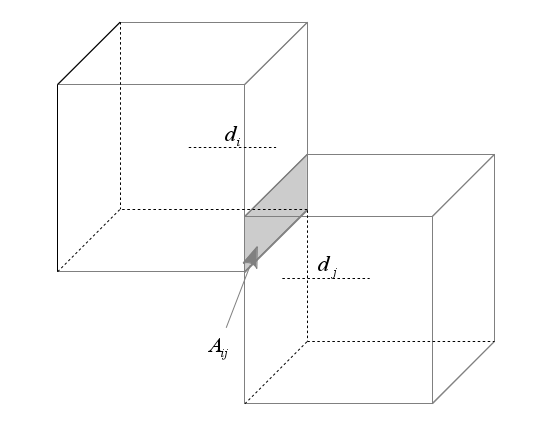
\includegraphics[width=6cm]{pics/link_2.png}
\caption{Связь между блоками}
\end{center}
 \label{links}
\end{figure}
\end{itemize}

Итак, имеем:
\begin{eqnarray}
  {F_{diff}}_c ( p, \ N_1, \dots ,  N_{n_c} ) =\sum\limits_{P = O, W, G}{T_dS_p\xi_pD_{c,P}({x_{c,P}}_i - {x_{c,P}}_j})
\end{eqnarray}
\newpage
\subsubsection{Система алгебраических уравнений}
Таким образом, задача сводится к системе алгебраических уравнений вида 
\begin{equation}
\bf F (\bf p, \bf N_1, \dots , \bf N_{n_c} ) = 0
\end{equation}
где $\bf p = (p^i), \bf N_c = (N_c^i)$ -- векторы значений давления и молярных плотностей в блоках сетки. Для решения системы нелинейных уравнений $F(x) = 0, x = (\bf p, \bf N)$ применяется стандартный метод Ньютона (см. ~\cite{Aziz}, ~\cite{Chen})

\begin{equation}
x_{m+1} = x_m - (\frac{\partial F(x_m)}{\partial x})^{-1}\,F(x_m)
\end{equation}

Здесь $\partial F (x_m) / \partial x$ -- отображение (матрица) 
$\bf R ^ {n_c \cdot (2 \cdot K)} \rightarrow \bf R ^ {n_c \cdot (2 \cdot K)} \times \bf R ^ {n_c \cdot (2 \cdot K)}$, где 
$\bf K$ -- число блоков. На каждом шаге метода Ньютона необходимо решать систему с несимметричной матрицей 
$\partial F (x_m) / \partial x$, т.е задача сводится к решению системы линейных уравнений 

\begin{eqnarray}
\label{DP_SLU}
Ax = r
\end{eqnarray}
матрица которой есть якобиан метода Ньютона. Матрицу A можно рассматривать как матрицу, элементами которой являются блоки размера 
$n_c \times n_c$. Значение $n_c$ варьируется в зависимости от типа задачи от 2 до 50 (см. ~\cite{Chen}, ~\cite{Aziz}, ~\cite{BogachevJabitskii-ILU}).
\\ \\

$$A_{ij} = \frac{\partial {{F_{flow}}_i}}{\partial x^j} + \frac{\partial {F_{Q}}_i}{\partial x^j} + \frac {\partial {F_{diff}}_i}{\partial x^j}\quad c=1,\dots,n_c \qquad$$
где ${F_{flow}}_i$ -- фильтрационная часть, ${F_{Q}}_i$ -- химическая реакция в блоке, ${F_{diff}}_i$ -- диффузионная часть блока $i$.
Обозначим количество связей с другими блоками за $N_l$. \\
Тогда $\frac {\partial {F_{diff}}_i}{\partial x^k}$ имеет следующий вид:
$$\frac {\partial {F_{diff}}_i}{\partial x^k} = \sum\limits_{j=1}^{N_l}\frac {\partial {F_{diff}}_{ij}}{\partial x^k}$$
где ${F_{diff}}_{ij}$ --- диффузионный переток между блоком $i$ и $j$.\\
Производная имеет следующий вид:
\begin{eqnarray}
\frac {\partial {F_{diff}}_{ij}}{\partial x^k} &=& \sum\limits_{P = O, W, G}{T_d \frac{\partial S_p}{\partial x^k}\xi_pD_{c,P}({x_{c,P}}_i - {x_{c,P}}_j}) \nonumber
\\&+& T_dS_p\frac {\partial \xi_p}{\partial x^k} D_{c,P}({x_{c,P}}_i - {x_{c,P}}_j)  \nonumber
\\&+& T_dS_p\xi_pD_{c,P}\frac {\partial({x_{c,P}}_i - {x_{c,P}}_j)}{\partial x^k}
\end{eqnarray}
где
\begin{eqnarray}
\frac{\partial S_p}{\partial x^k} &=& \begin{cases} \frac{\partial S_i}{\partial x^k}, & S_i < S_j\\ \frac{\partial S_j}{\partial x^k}, & S_i > S_j \end{cases} \nonumber \\
\end{eqnarray}
Заметим, что одна из производных равна нулю, поскольку $S_k$ может явно зависеть только от переменных своего блока.\\ \\
Аналогично вычисляется и производная по $\xi_p$:
\begin{eqnarray}
\frac{\partial \xi_p}{\partial x^k} &=& \begin{cases} \frac{\partial xi_i}{\partial x^k}, & {x_{c,P}}_i > {x_{c,P}}_j\\ \frac{\partial \xi_j}{\partial x^k}, & {x_{c,P}}_i < {x_{c,P}}_j \end{cases} \nonumber \\
\end{eqnarray}

\section{Диффузия в модели метана угольных пластов}
\subsection{Физическая модель}
Метан угольных пластов содержится в угленосных отложениях. Он формируется в результате биохимических и физических процессов в ходе преобразования растительного материала в уголь.
Для увеличения газоотдачи применяется технология гидроразрыва пласта --- создание высокопроводимой трещины в целевом пласте для обеспечения притока добываемого газа.

\subsection{Математическая модель}
\subsubsection{Двойная пористость}
Для расчета этой задачи используется модель двойной пористости. Среда нашего резервуара состоит из двух типов пород: низкопроницаемый уголь (т.н. матрица) и высокопроницаемая трещина.
Залежи метана находятся в матричной породе и получить их непосредственно из нее невозможно, только через прилегающую трещину. Таким образом, модель резервуара представляет из себя две сплошные среды : матрицу и трещину, где матрица -- носитель ресурса, а трещина -- система, по которой этой ресурс может течь по породе резервуара. На рис.~\ref{DPscheme}  схематично представлена двойная среда с поровыми (матричными) блоками, разделенными трещинами (см. ~\cite{Aziz}).

\begin{figure} [!h]
\begin{center}
\caption{Схема двойной среды}
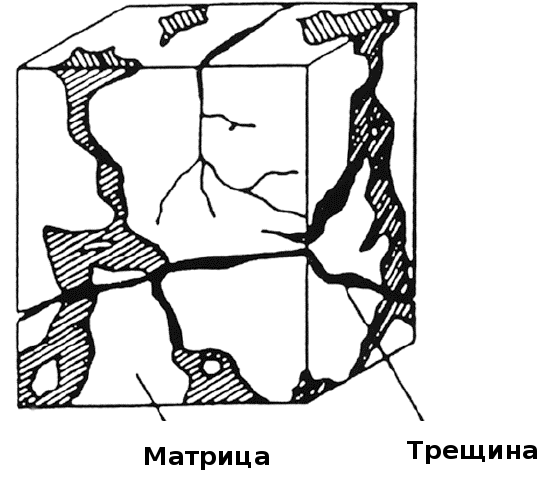
\includegraphics[width=0.4\textwidth]{pics/DPscheme_Aziz.png}
\end{center}
 \label{DPscheme}
\end{figure}

При моделировании двойной среды для каждого блока вводят два давления : давление газа в матрице и давление газа в трещине. Также учитывается массообмен между матрицей и трещиной. Таким образом, один и тот же блок реального резервуара раскладывается на два блока: один матрицы, другой трещины (см ~\cite{Chen}).

\begin{figure}[!h]
\begin{center}
\caption{Блоки матрицы и трещины}
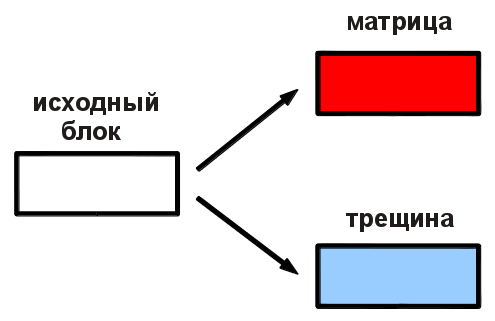
\includegraphics[width=8cm]{pics/matrixfracture.png}
\end{center}
\label{DPblocks}
\end{figure}


При этом особенности модели двойной пористости заключаются в следующем: 

\begin{itemize}
\item Каждый блок матрицы обязан быть связан с соответствующим блоком трещины.

\item Если блок матрицы активен, то обязан быть активен соответствующий блок трещины. Обратное неверно, т.е при активной трещине соответствующий блок матрицы может быть неактивен.

\item Активный блок матрицы может иметь связь (т.е возможен поток) только с соответствующим блоком трещины (т.е запрещена связь  напрямую матрица - матрица).

\item Внешние источники (скважины) подключены только к блокам трещины.
\end{itemize}

С учетом особенностей этой модели, уравнения для модели двойной пористости перепишутся в виде: (см. например ~\cite{Aziz}, ~\cite{Chen}): 

\begin{eqnarray}
\text{Для трещины : } \nonumber \\ \nonumber
  \dfrac{\partial}{\partial t} \left(\phi N_c\right) &= \nonumber
  & \Div\sum\limits_{P = O, W, G} x_{c,P} \xi_P \Bigl({\bf k} \dfrac{k_{rP}}{\mu_P}(\nabla p_P - \gamma_P \nabla D)\Bigr)+\nonumber\\
  & &\quad +q_c + q_{FM}, \quad c=1,\dots,n_c \nonumber\\
  p_o - p_g &= &P_{cog},  \nonumber\\
  p_o - p_w &= &P_{cow}, \nonumber \\
  S_w + S_o + S_g &= &1. \nonumber \\
\text{Для матрицы : }\nonumber \\
  \dfrac{\partial}{\partial t} \left(\phi N_c\right) &=& q_{MF}, \quad c=1,\dots,n_c  \nonumber\\
  p_o - p_g &= &P_{cog}, \nonumber\\
  p_o - p_w &= &P_{cow}, \nonumber \\
  S_w + S_o + S_g &= &1. \nonumber
\end{eqnarray}
где $q_{FM}$ -- перетоки между матрицей и трещиной.\\
Проницаемость между матрицей и трещиной является нулевой. Газ может попасть в трещину только диффундируя через связь с трещиной.\\
Поэтому из закона Фика (\ref {Fick}) следует:
\begin{eqnarray}
\text{Для трещины : } \nonumber \\ \nonumber
  \dfrac{\partial}{\partial t} \left(\phi N_c\right) &= \nonumber
  & \Div\sum\limits_{P = O, W, G} x_{c,P} \xi_P \Bigl({\bf k} \dfrac{k_{rP}}{\mu_P}(\nabla p_P - \gamma_P \nabla D)\Bigr)+\nonumber\\
  & &\quad +q_c + \Div J_c, \quad c=1,\dots,n_c \nonumber\\
  p_o - p_g &= &P_{cog},  \nonumber\\
  p_o - p_w &= &P_{cow}, \nonumber \\
  S_w + S_o + S_g &= &1. \nonumber \\
\text{Для матрицы : } \nonumber\\
  \dfrac{\partial}{\partial t} \left(\phi N_c\right) &=& - \Div J_c, \quad c=1,\dots,n_c  \nonumber\\
  p_o - p_g &= &P_{cog}, \nonumber\\
  p_o - p_w &= &P_{cow}, \nonumber \\
  S_w + S_o + S_g &= &1. \nonumber
\end{eqnarray}

\subsection {Дискретизация уравнений}

Диффузионный член $\Div J_c$ приводится к дискретному виду аналогично пункту ~\ref{numerical}. В модели метана угольных пластов рассматривают диффузию исключительно газовой фазы.

$$ {F_{diff}}_c ( p, \ N_1, \dots ,  N_{n_c} ) =T_dS_p\xi_pD_{c,P}({x_{c,GAS}}_i - {x_{c,GAS}}_j)$$

Концентрация адсорбированной компоненты $i$ на поверхности выражается через изотерму Ленгмюра: (см. ~\cite{ArriYee})

\begin{eqnarray}
L_i (p, y_i) = \theta \frac {P_s}{RT_s}\frac{V_i\frac{y_ip}{P_i}}{1 + \sum\limits_{j=1}^{N_c}{\frac{y_jp}{P_j}}}
\end{eqnarray}
где
\begin{itemize}
\item $p$ -- давление в блоке
\item $y_c = y_c(p, \bf N)$ -- молярная доля компоненты $c$ в газовой фазе,
\item $P_s = const$ -- давление при стандартных условиях
\item $T_s = const$ -- температура при стандартных услоиях
\item $R = const$ -- универсальная газовая постоянная
\item $V_i = const$ -- объемная константа Ленгмюра 
\item $P_i = const$ -- константа давления Ленгмюра
\end{itemize}

Концентрацию со стороны матрицы возьмем $y_i$, со стороны трещины возьмем $L_i$.
Диффузивность в этой модели рассчитываетя по формуле $T_d=V\sigma$, где $\sigma$ - константа.

С учетом этого, закон Фика примет следующий вид:
\begin{eqnarray}
{F_{diff}}_c = T_dD_{c,i}(N_i - \rho_{rock}L_i)
\end{eqnarray}
В случае, если разность потенциалов $N_i -\rho_{rock}L_i$ отрицательна, то имеет место т.н. реадсорбция, то есть уголь продолжает насыщаться газом.\\
Поскольку протекающая диффузия прямо пропорциональна минимальной насыщенности, то мы берем $S_{gas}$ в трещине, т.к. $S_{gas}$ в угле равен единице. Заметим, что поровый объем трещины в модели метана угольных пластов делят между собой две фазы: вода и газ. Добыча метана начинается с откачки воды из трещин. Понижение насыщенности водой приводит к повышению $S_{gas}$ и, соответственно, к повышению добычи метана. Также в уравнение добавляют коэффициент реадсорбции, чтобы можно было контролировать или полностью убрать этот эффект.
\begin{eqnarray}
F_c = T_dR_fS_{gas}D_{c,i}(N_i - \rho_{rock}L_i)
\end{eqnarray}
\section{Реализация}
На основе приведенного алгоритма была написана работающая программа на языке C++ для параллельных вычислений на системах как с общей, так и с распределенной памятью (см. ~\cite{Bogachev}). Программа включена в состав Российского гидродинамического симулятора tNavigator. При этом используется решение задачи (\ref{filtration_1})---(\ref{filtration_4}), реализованное в tNavigator. За основу взято готовое решение системы линейных уравнений (\ref{DP_SLU}). Оно проводится итерационным алгоритмом BiCGSTAB (см. ~\cite{Saad}), в котором в качестве предобуславливателя берутся блочные аналоги ILU разложений (см. ~\cite{Saad}, блочный вариант см. ~\cite{BogachevJabitskii-ILU}).

\subsection{Основные сложности multi-thread и MPI-реализации}
Приведенный алгоритм реализован и включен в гибридную работающую параллельную программу на системах с разделенной памятью. \\
Каждый логический процесс вычисляет значения в своих строках матрицы по посчитанным значениям свойств смеси в блоках сетки
и их частным производным по $p$, $\bf N$.\\
При моделировании необходимо было решать следующие проблемы:
\begin{itemize}
\item решение проблем с локальной индексацией текущего процесса.
\item доступ к элементам другого процесса.
\end{itemize}
\newpage
\subsection{Отладка}
Отладка значений элементов якобиана происходила следующим образом: 
\begin{itemize}
 \item Подсчет производных явным способом, через частные производные свойств смеси по главным переменным $p$, $\bf N$. 
 \item Подсчет производных численно, без использования частных производных свойств смеси. Все свойства дополнительно рассчитываются 
 при значении переменной, сдвинутой на малую величину $h$.
 \item Проверяется соблюдение асимптотики $O(h)$. \\ \\ \\
\end{itemize}
Для отладки значений свойств смеси в блоках с учетом диффузии были реализованы:
\begin{itemize}
\item Карты межблочных перетоков для каждой компоненты.
\item Карта диффузивности.
\item Карта изотерм Ленгмюра.
\item Карта угольных регионов.
\item Карта плотности угля.
\item Графики перетоков между отчетными регионами.
\end{itemize}

\newpage
\section{Численные результаты}
\subsection {Тестовая модель для диффузии 2х1х1}
Итак, рассмотрим простейшую модель, состоящую из двух блоков. В модели присутствуют 5 компонент.
Проницаемость между блоками нулевая. Состав смеси в блоках задан следующей таблицей концентраций:
\begin{table}[!h]
\caption{Концентрации компонент}
\begin{center}
\begin{tabular}{|c|c|}
\hline
1 & 2 \\
\hline
0.5 & 0.0 \\
\hline
0.0 & 0.5 \\
\hline
0.25 & 0.25 \\
\hline
0.25 & 0.25 \\
\hline
0.0 & 0.0 \\
\hline
\end{tabular}
\end{center}
\end{table}

\subsubsection{Давление}
Давление в обоих блоках в начальный момент времени выровнено. Напомним, что в качестве потенциала фильтрации выступает именно градиент давления.

\begin{figure} [!h]
\begin{center}
\caption{Карта давления на 1000 шаге по времени}
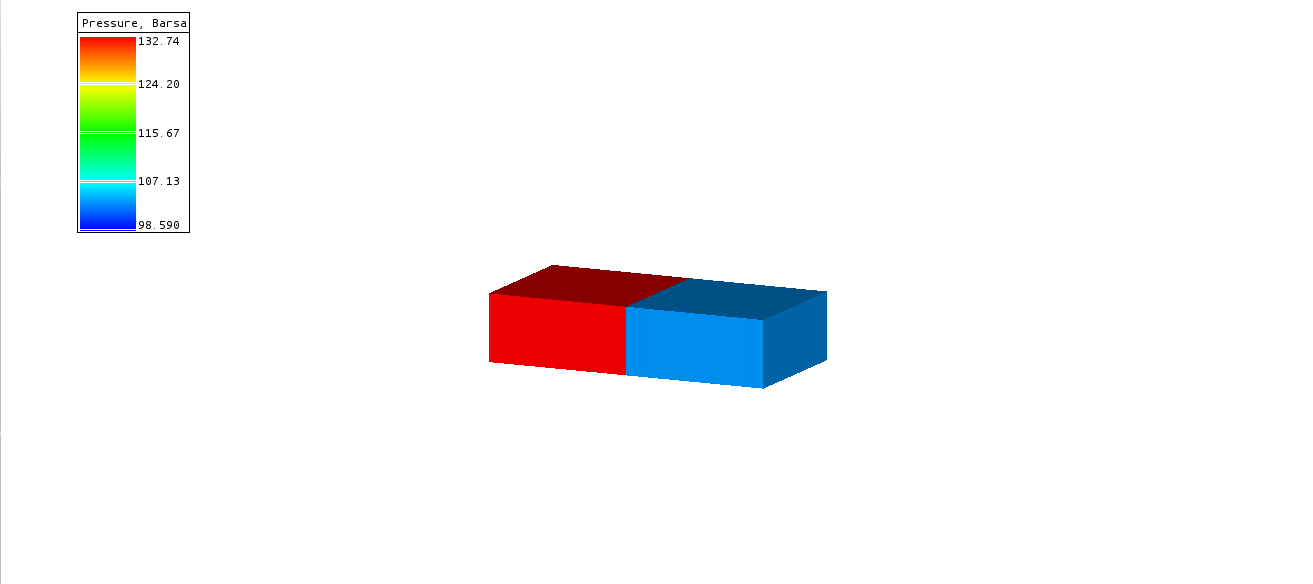
\includegraphics[width=1.2\textwidth]{pics/pressuret211_1.png}
\end{center}
\end{figure}

Таким образом, процесс диффузии теоретически может приводить к перепадам давления в изолированных друг от друга блоках.
\newpage
\subsubsection{Скорость выравнивания концентраций}
Проведем тест с включенной диффузией одной компоненты.\\
Зададим следующие коэффициенты диффузии:
\begin{table}[!h]
\caption{Коэффициенты диффузии}
\begin{center}
\begin{tabular}{|c|c|c|c|c|}
\hline
comp 1 & comp 2 & comp 3 & comp 4 & comp 5\\
\hline
1 & 0 & 0 & 0 & 0\\
\hline
\end{tabular}
\end{center}
\end{table}

Динамику выравнивания концентраций можно посмотреть на следующей таблице:

\begin{table}[!h]
\caption{Таблица концентраций первой компоненты 'comp 1'}
\begin{center}
\begin{tabular}{|c|c|c|}
\hline
\backslashbox{step}{block} & 1 & 2 \\
\hline
0 & 0.5 & 0.0 \\
\hline
50 & 0.4048 & 0.1808 \\
\hline
100 & 0.3540 & 0.2378 \\
\hline
150 & 0.3250 & 0.2635 \\
\hline
200 & 0.3091 & 0.2760 \\
\hline
250 & 0.3003 & 0.2825 \\
\hline
300 & 0.2956 & 0.2859 \\
\hline
350 & 0.2930 & 0.2877 \\
\hline
400 & 0.2916 & 0.2887 \\
\hline
450 & 0.2908 & 0.2893 \\
\hline
680 & 0.2899 & 0.2899 \\
\hline
\end{tabular}
\end{center}
\end{table}

Теперь рассмотрим две активные компоненты.
Зададим следующие коэффициенты диффузии:
\begin{table}[!h]
\caption{Коэффициенты диффузии}
\begin{center}
\begin{tabular}{|c|c|c|c|c|}
\hline
comp 1 & comp 2 & comp 3 & comp 4 & comp 5\\
\hline
1 & 1 & 0 & 0 & 0\\
\hline
\end{tabular}
\end{center}
\end{table}
\\
Проследим за выравниванием концентраций. Значения концентраций на различных шагах даны в следующих таблицах:
\newpage
\begin{table}[!h]
\caption{Таблица концентраций второй компоненты 'comp 1'}
\begin{center}
\begin{tabular}{|c|c|c|}
\hline
\backslashbox{step}{block} & 1 & 2 \\
\hline
0 & 0.5 & 0.0 \\
\hline
50 & 0.3604 & 0.1989 \\
\hline
100 & 0.3109 & 0.2627 \\
\hline
150 & 0.2949 & 0.2833 \\
\hline
200 & 0.2903 & 0.2894 \\
\hline
211 & 0.2899 & 0.2899 \\
\hline
300 & 0.2911 & 0.2890 \\
\hline
350 & 0.2909 & 0.2892 \\
\hline
400 & 0.2906 & 0.2894 \\
\hline
722 & 0.2899 & 0.2899 \\
\hline
\end{tabular}
\end{center}
\end{table}

\begin{table}[!h]
\caption{Таблица концентраций второй компоненты 'comp 2'}
\begin{center}
\begin{tabular}{|c|c|c|}
\hline
\backslashbox{step}{block} & 1 & 2 \\
\hline
0 & 0.5 & 0.0 \\
\hline
50 & 0.3200 & 0.1249 \\
\hline
100 & 0.2549 & 0.1755 \\
\hline
150 & 0.2297 & 0.1952 \\
\hline
200 & 0.2194 & 0.2032 \\
\hline
250 & 0.2148 & 0.2066 \\
\hline
300 & 0.2126 & 0.2083 \\
\hline
350 & 0.2115 & 0.2091 \\
\hline
400 & 0.2109 & 0.2095 \\
\hline
710 & 0.2101 & 0.2101 \\
\hline
\end{tabular}
\end{center}
\end{table}

Можно заметить, что равновесие для первой компоненты наступило гораздо раньше -- уже на 211 шаге. Однако общее равновесие системы наступило несколько позже первого случая.
\newpage
\subsection {Тестовая модель для диффузии 9x9x9}
Модель представляет из себя равномерную модель с одинаковыми блоками и одну нагнетательную скважину, расположенную в центре.
Проницательность $PERM_x = PERM_y = PERM_z = 0$. Забойное давление скважины  $p_{well} = 500$ Бар. Концентрации $x_{1,GAS} = 0.26$ во всех блоках. Коэффициенты диффузии $D_{1,gas} = 1$, $D_{c,p} = 0 \quad\forall c\neq 1, p\neq GAS$.\\
Динамику можно проследить по следующим картам давления:

{{\center{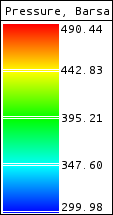
\includegraphics[width=70pt]{pics/pressure999.png}}  \\
\begin{minipage}[h]{0.4\linewidth}
{\center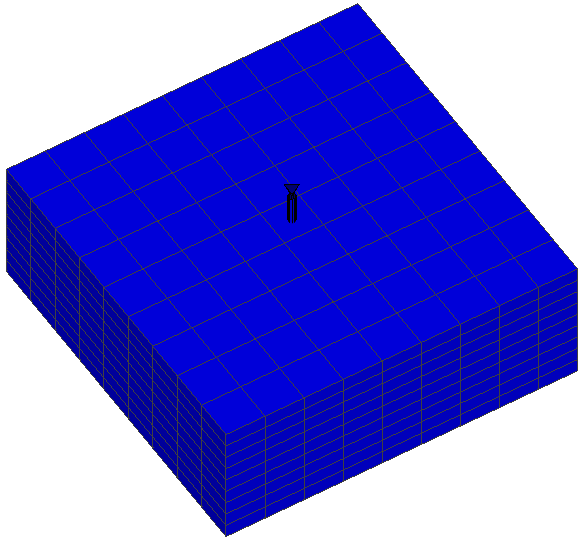
\includegraphics[width=1\linewidth]{pics/pressure999_0.png}} Давление на 0 шаге по времени \\
\end{minipage}
\hfill
\begin{minipage}[h]{0.4\linewidth}
{\center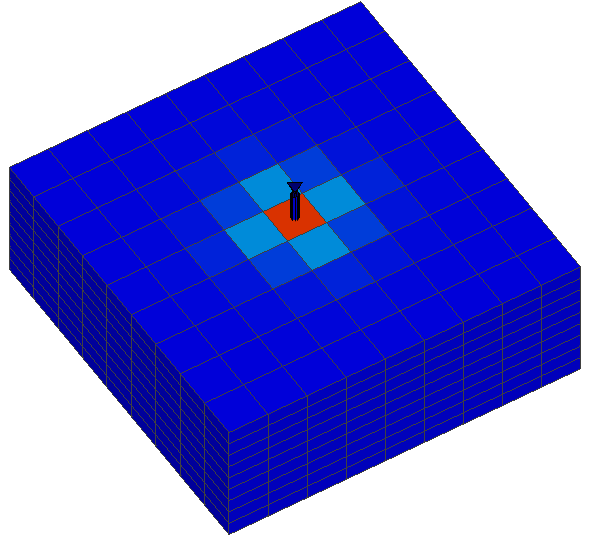
\includegraphics[width=1\linewidth]{pics/pressure999_15.png}} \\Давление на 15 шаге по времени
\end{minipage}
\vfill
\begin{minipage}[h]{0.4\linewidth}
{\center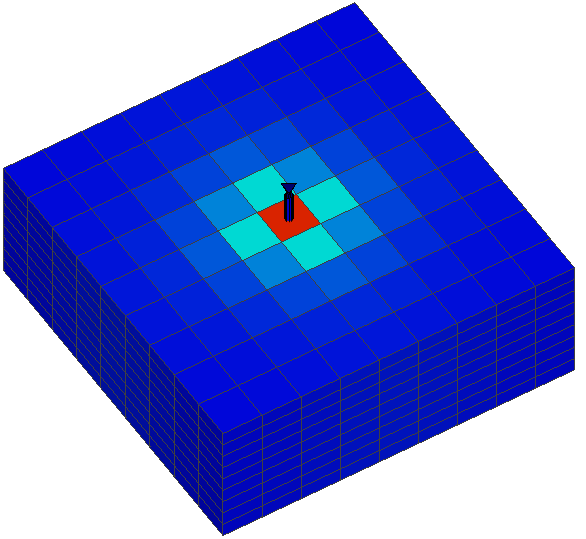
\includegraphics[width=1\linewidth]{pics/pressure999_50.png}} Давление на 50 шаге по времени \\
\end{minipage}
\hfill
\begin{minipage}[h]{0.4\linewidth}
{\center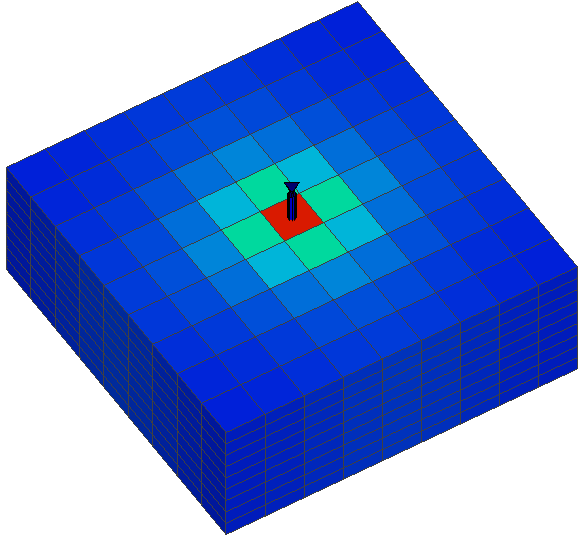
\includegraphics[width=1\linewidth]{pics/pressure999_100.png}} Давление на 100 шаге по времени \\
\end{minipage}
}
\newpage
\subsection {Тестирование диффузии на реальных геологических моделях. Влияние на производительность.}
Добавление в уравнение диффузионного члена, разумеется, замедляет сходимость метода Ньютона. Производительность моделей с диффузией была протестирована на реальных геологических моделях.

\begin{table}[!h]
\caption{Влияние на производительность}
\begin{center}
\begin{tabular}{|c|c|c|c|c|c|c|c|}
\hline
№ & Active cells & Comps & N & CPU default & CPU with diffusion & abs & \% \\
\hline
1 & 14461 & 7 & 101227 & 00.00.49 & 00.00.51 & +00.00.02 & +4.0\% \\
\hline
2 & 231251 & 3 & 693753 & 00.08.02 & 00.08.12 & +00.00.10 & +2.1\% \\
\hline
3 & 2510146 & 3 & 7530438 & 01.31.53 & 01.36.24 & +00.04.31 & +4.9\% \\
\hline
4 & 182755 & 3 & 548265 & 00.35.57 & 00.37.27 & +00.01.30 & +4.1\% \\
\hline
5 & 27000 & 3 & 81000 & 00.03.24 & 00.03.33 & +00.00.09 & +4.4\% \\
\hline
6 & 61179 & 3 & 183537 & 00.03.53 & 00.04.01 & +00.00.08 & +3.4\% \\
\hline
\end{tabular}
\end{center}
\end{table}
где
\begin{itemize}
\item Active cells --- количество активных блоков в модели
\item Comps --- количество компонент
\item N --- размерность якобиана
\end{itemize}

\section{Результаты}
Была написана работающая программа на языке С++ для параллельных вычислений как с общей, так и с распределенной памятью для моделирования:
\begin{itemize}
\item задачи фильтрации с учетом диффузии в моделях черной нефти. 
\item задачи фильтрации с учетом диффузии в композиционных моделях.
\item задачи фильтрации с учетом диффузии в моделях метана угольных пластов.
\end{itemize}
Были проведены тесты на реальных геологических моделях и выявлены совпадения результатов с известными симуляторами нефтяных месторождений. Алгоритм реализован на С++ для multi-thread и MPI-гибридных систем и включен в промышленный гидродинамический симулятор tNavigator.


\newpage

\ifx\undefined\BibEmph\def\BibEmph#1{#1}\else\fi
\ifx\undefined\href\def\href#1#2{#2}\else\fi
\ifx\undefined\url\def\url#1{\texttt{#1}}\else\fi
\ifx\undefined\urlprefix\def\urlprefix{URL: }\else\fi
\ifx\undefined\BibUrl\def\BibUrl#1{\urlprefix\url{#1}}\else\fi
\ifx\undefined\BibUrlDate\long\def\BibUrlDate#1{({%
\cyr\cyrd\cyra\cyrt\cyra\ 
\cyro\cyrb\cyrr\cyra\cyrshch\cyre\cyrn\cyri\cyrya}: #1)}\else\fi
\ifx\undefined\BibAnnote\long\def\BibAnnote#1{#1}\else\fi
\begin{thebibliography}{1}
\addcontentsline{toc}{section}{\bibname}
\def\selectlanguageifdefined#1{
\expandafter\ifx\csname date#1\endcsname\relax
\else\language\csname l@#1\endcsname\fi}

\bibitem{Aziz}
\selectlanguageifdefined{english}
\BibEmph{Aziz~K., Settari~A.} Petroleum reservoir simulation.
  \BibEmph{London : Applied Science Publishers}.
\newblock 1979.

\bibitem{Chen}
\selectlanguageifdefined{english}
\BibEmph{Chen~, Zhangxin and Huan, Guanren and Ma, Yuanle} 
Computational Methods for Multiphase Flows in Porous Media (Computational Science and Engineering 2)~//
  \BibEmph{Society for Industrial and Applied Mathematics, Philadelphia, PA, USA}
\newblock 2006
\newblock {\cyr\CYRT.}~11.
\newblock {\cyr\CYRS.}~193--197.



\bibitem{Saad}
\selectlanguageifdefined{english}
\BibEmph{Yousef Saad}
Iterative Methods for Sparse Linear Systems, Second Edition
  \BibEmph{Society for Industrial and Applied Mathematics, Philadelphia, PA, USA}
\newblock 2003

\bibitem{Bogachev}
\selectlanguageifdefined{russian}
\BibEmph{Богачев~К.~Ю.}
	Основы параллельного программирования.
  \BibEmph{Москва. Бином. Лаборатория знаний}.
\newblock 2010.
	
\bibitem{ClusterBalancingArticle}
\selectlanguageifdefined{russian}
\BibEmph{Богачев~К.~Ю., Климовский~А.~А., Миргасимов~А.~Р., Семенко~А.~Е.}
  Балансировка загруженности узлов кластера при расчете задачи фильтрации~//
  \BibEmph{Вычислительные методы и программирование}.
\newblock 2011.
\newblock {\cyr\CYRT.}~12.
\newblock {\cyr\CYRS.}~70--73.

\bibitem{BogachevMelnichenko}
\selectlanguageifdefined{russian}
\BibEmph{Богачев~К.~Ю., Мельниченко~Н.~С.} О пространственной аппроксимации
  методом подсеток для задачи фильтрации вязкой сжимаемой жидкости в пористой
  среде~// \BibEmph{Вычислительные методы и программирование}.
\newblock 2008.
\newblock {\cyr\CYRT.}~9, {\cyr\textnumero}~2.
\newblock {\cyr\CYRS.}~42--50.

\bibitem{BogachevJabitskii-ILU}
\selectlanguageifdefined{russian}
\BibEmph{Богачев~К.~Ю., Жабицкий~Я.~В.} Блочные предобусловливатели класса ILU
  для задач фильтрации многокомпонентной смеси в пористой среде~//
  \BibEmph{Вестн. Моск. ун-та. Математика. Механика}.
\newblock 2009.
\newblock {\cyr\textnumero}~5.
\newblock {\cyr\CYRS.}~19--25.

\bibitem{BogachevJabitskii-KaporinKonshin}
\selectlanguageifdefined{english}
\BibEmph{Богачев~К.~Ю. Жабицкий~Я.~В.} 
Метод Капорина-Коньшина параллельной реализации блочных предобуславливателей для несимметричных матриц в задачах фильтрации многокомпонентной смеси в пористой среде~//
  \BibEmph{Вестн. Моск. ун-та. Математика. Механика}.
\newblock 2010.
\newblock {\cyr\textnumero}~1,
\newblock {\cyr\CYRS.}~46--52.


\bibitem{BogachevMirgasimov}
\selectlanguageifdefined{russian}
\BibEmph{Богачев~К.~Ю., Миргасимов~А.~Р.} Об оптимизации вычислительных
  приложений для многопроцессорных систем с общей неоднородной памятью~//
  \BibEmph{Вычислительные методы и программирование}.
\newblock 2010.

\bibitem{ArriYee}
\selectlanguageifdefined{english}
\BibEmph{Arri, ~L.~E., Yee, ~D., Morgan, ~W.~D., and Jeansonne, ~N.~W. } Modeling Coalbed Methane Production with Binary Gas Sorption.

\bibitem{Fick}
\selectlanguageifdefined{english}
\BibEmph{Fick ~A.} Ueber Diffusion (1855).

\end{thebibliography}

\end{document}